\chapter{Mass Transport}

\section{多组分质量传递基本概念}

对多组分流体混合物而言,质量的关系为$ m=\sum m_i $,将质量浓度(\si{\kilogram\per\meter\cubed})定义为:

\[\rho_i = \frac{m_i}{V} \]

混合物的密度为全部物质的质量浓度之和:

\[\rho = \sum\rho_i \]

类似地,混合物的物质的量(\si{\mole})、质量分数($ \sum \omega_i = 1 $)、摩尔分数($ \sum x_i = 1 $)分别定义为:

\[ n_i=\frac{m_i}{M_i} \]
\[ \omega_i = \frac{m_i}{m} \]
\[ x_i = \frac{n_i}{n} \]

并且有如下转换关系:

\[\rho_i = \rho\omega_i = \rho\frac{M_i}{M}x_i \]

\[c_i = \frac{n_i}{V} = \frac{m_i/M_i}{V} = \frac{\rho_i}{M_i}  = \frac{p_i}{RT} \]

质量分数$ \omega_i $还可定义为溶质的质量浓度$ \rho_i $和溶液的质量浓度$ \rho $之比:

\[\omega_i = \frac{\rho_i}{\rho} =\frac{c_i M_i}{\rho}\]

那么,显然,浓度$ c_i $和质量分数有如下转换关系:

\[ c_i = \frac{n_i}{V} = \frac{m_i}{M_i V} = \frac{\rho_i V}{M_i V} = \frac{\rho\omega_i V}{M_i V} = \frac{\rho\omega_i}{M_i}\]

混合物的等效摩尔质量(\si{\kilogram\per\mole})定义为:

\[ M = \sum M_i x_i \]

如果气体混合物是理想气体,则满足:

\[ PV=nRT \]
\[ PV=mR_m T \]

其中$ R_m $是混合物气体参数,定义为:

\[ R_m = \frac{n}{m}R = \frac{R}{M} \]

Dalton定律,在组分之间不发生化学反应的前提下,理想气体混合物的压强等于各组分的分压之总和,组分的摩尔分数等于分压与总压之比。其中气体$ i $的分压为$ P_i $。

\[ p=\sum p_i \]
\[x_i = \frac{p_i}{p}\]

Raoult定律,描述了溶液的蒸气压与其浓度的关系。在一定温度下,理想溶液内每一组分的蒸气压等于该组分的摩尔分数与其作纯溶剂时的蒸气压的乘积,且总的蒸气压等于各组分的蒸气压之和。

\begin{equation}
p = \sum p_i^* x_i
\end{equation}


\section{质量守恒}

对一个体积为$ \Delta x \Delta y \Delta z $的控制体而言,质量守恒可以表示为\textbf{控制体的净流出+控制体内质量的净积累率=0},数学描述如下:

\begin{equation}
\iint_{cs} \rho(\bm{u\cdot n})dA + \frac{\partial }{\partial t} \iiint_{cv}\rho dV = 0
\end{equation}

整理为矢量形式,其中,反应速率单位为\si{\kg\per\meter\cubed\per\second},

\begin{equation}
\nabla \cdot \rho\mathbf{u} + \frac{\partial \rho}{\partial t} = R
\end{equation}

考虑到$ c=\rho/M $,可整理为关于摩尔浓度的质量守恒方程,其中体积净反应速率单位为\si{\mole\per\meter\cubed\per\second},

\begin{equation}
\nabla \cdot c\mathbf{u} + \frac{\partial c}{\partial t} = R
\end{equation}

考虑到系统内存在的扩散效应,质量守恒方程为,

\begin{equation}
\frac{\partial c}{\partial t} + \nabla \cdot c\mathbf{u} - \nabla\cdot(D\nabla c) = R
\end{equation}

对一个纯扩散系统,质量守恒方程形式为经典的Fick第二定律,

\begin{equation}
\frac{\partial c}{\partial t} = D\nabla^2 c
\end{equation}

求解质量传递方程需要给定的边界条件一般分为四类:

\begin{enumerate}
\item 指定浓度,即$ c_i = c $
\item 指定通量,一般为表面反应通量,即$ N=R_s $,单位\si{\mole\per\meter\squared\per\second}
\item 零梯度,一般为不可渗透边界和对称面,$ \frac{\partial c}{\partial t}=0 $
\item 指定对流传质通量,一般为边界层内的质量传递通量,$ N=h(c_s-c_{bulk} ) $
\end{enumerate}

\section{对流传质}

这里所说的对流传质(Convective mass transfer)涉及到物质在边界表面和移动流体之间的传递现象,其质量传递通量与对流传质系数有关,确定对流传质系数不是一件容易的事,传质系数与流体性质、流动特性以及系统的几何形状有关。对流传质的速率类似于Newton冷却定律,

\begin{equation}
N=h\Delta c
\end{equation}

边界层理论认为,流体在表面的平行流动会产生速度分布,流体在表面速度为0,边界层边缘接近本体速度,因此流体到表面的质量传递基本只靠分子扩散,即:

\[N=-D\frac{d(c-c_{s})}{dy} = h(c_s-c_{bulk})\]

其中,$ c_s $为表面浓度。

重整形式,并乘上特征长度$ L $,得到Sherwood数:

\[Sh = \frac{hL}{D} = \frac{-d(c-c_s)/dy}{(c_s-c_{bulk})/L}\]

\section{分子扩散}

Fick第一定律表明,分子扩散通量与浓度梯度成正比,

\begin{equation}\label{Fick's_1}
N = -D\nabla c
\end{equation}

\section{Mass diffusivity}
扩散系数分为三类,热扩散系数$ \alpha $、质量扩散系数$ D $、动量扩散系数$ \nu $,单位均为\si{\square\meter\per\second}。三类扩散系数及其关联物理量,如粘度$ \mu $、热导率$ k $均可以通过Elementary Kinetic Theory或者Chapman–Enskog Theory估算,详情参加文献\cite{yan2010CVD}。

\[J=-D_{AB}\frac{dc_A}{dy}\]
\[q=-\alpha\frac{d(\rho c_p T)}{dy} = -k\frac{dT}{dy} \]
\[\tau = -\nu\frac{d(\rho u)}{dy} = -\mu\frac{du}{dy}\]

定义Schmidt数为$ Sc=\nu/D $,根据动力学理论,理想气体的$ Sc=1 $,故$ Sc $数其主要用来表征气体与理想气体的偏差(即表征气体的非理想性)。气体的Schmidt数通常在$ 0.2\sim 3 $,液体的Schmidt通常$ >40000 $。

浓度梯度引起分子扩散,通常化合物在空气中的扩散系数为在水中的扩散系数的1000倍左右。气体的扩散系数在\num{e-6}到\num{e-5}~\si{\square\meter\per\second},对气体而言,根据动力学理论可知,气体的扩散系数与温度和压力相关,关系通常为$ f(T^n/p) $(通常$ n=3/2 $),气体的扩散系数通常随温度升高或压力下降而增大。实际上,由于气体的非理想性,$ n $通常要更大,例如水汽在空气中扩散,$ n=2.072(250\si{\kelvin}<T<459\si{\kelvin}) $。液体和固体的扩散系数与浓度紧密相关,并且通常随温度增大而增大,液体的扩散系数在\num{e-10}到\num{e-9}~\si{\meter\squared\per\second}左右,固体的扩散系数一般在\num{e-14}到\num{e-10}~\si{\meter\squared\per\second}或更小。

对低压气体混合物而言,扩散系数$ D_{AB} $与压力$ p $成反比,与温度$ T $成正比,并且几乎与给定气体对的组成无关。

Sutherland, Jeans, Chapman和Cowling等人基于气体动力学理论(参见文献\footnote{Welty J R, Wicks C E, Rorrer G, et al. Fundamentals of momentum, heat, and mass transfer[M]. John Wiley \& Sons, 2009.}),导出预测扩散系数的模型。最简化的动力学模型把分子当作不是加分子间力的刚性球,且认为分子之间的碰撞事完全弹性的,对理想气体混合物总的组分A,其自扩散系数定义为,

\begin{equation}
D_{AA} = \frac{1}{3}\lambda u
\end{equation}

其中,$ \lambda $是分子的平均自由程,

\begin{equation}
\lambda = \frac{k_B T}{\sqrt{2}\pi\sigma_A^2 p}
\end{equation}

$ u $是物质A相对于分子平均速度的速度,

\begin{equation}
u = \sqrt{\frac{8k_B NT}{\pi M_A}}
\end{equation}

整理得到扩散系数,

\begin{equation}
D_{AA} = \frac{2T^{3/2}}{3\pi^{3/2}\sigma_A^2 p} \left( \frac{k_B^3 N}{M_A} \right)^{1/2}
\end{equation}

其中,$ N $是Avogadro常数(\num{6.022e23}),$ k_B $为Boltzmann常数,$ \sigma_A $为物质$ A $的Lennard–Jones分子直径。

使用相似的动力学理论可推算二元组分混合物的扩散系数,

\begin{equation}
D_{AB} = \frac{2}{3}\left(\frac{k_B}{\pi}\right)^{3/2}N^{1/2}T^{3/2}
\frac{\left(\dfrac{1}{2M_A}+\dfrac{1}{2M_B}\right)^{1/2}}
{p\left(\dfrac{\sigma_A+\sigma_B}{2}\right)^2}
\end{equation}

\subsection{二元组分的扩散}

二元系统的扩散系数可以使用对应态原理(corresponding states methods)来预测,可以以此来核算已知的实验数据或估算系统内未知的扩散系数,文献\footnote{B. E. Poling, J. M. Prausnitz, and J. P. O’Connell, The Properties of Gases and Liquids, 5th edition, McGraw-Hill, New York (2001), Chapter 11.}提供了多种预测扩散系数的方法。

传统的基于分子动力学理论的分子扩散模型没有考虑分子间力,Hirschfelder等人利用Lennard-Jones势来评估分子间力的影响,给出了非极性非反应分子气体对扩散系数的关联式,

\begin{equation}
D_{AB} = \frac{0.001858T^{3/2}\left(\dfrac{1}{M_A}+\dfrac{1}{M_B}\right)^{1/2}}{p\sigma_{AB}^2 \Omega_D}
\end{equation}

其中,$ D_{AB} $为二元扩散系数(\si{cm\squared\per\second});$ M $为分子质量;$ p $为压力(\si{atm});$ \sigma_{AB} $为平均碰撞直径(\si{\angstrom});$ \Omega_D $是一个碰撞积分,是温度和分子间势场的无量纲函数,参见文献\footnote{Welty J R, Wicks C E, Rorrer G, et al. Fundamentals of momentum, heat, and mass transfer[M]. John Wiley \& Sons, 2009.}查阅常用的一组碰撞积分的经验参数。

此外,比较常用的还有Fuller提出的一个经验关联式,形如$ D_{AB}=f(T^{1.75}/p) $,简单易用,误差不超过$ 10\% $。详情参见文献\cite{poling2001properties}。

\begin{equation}
D_AB=\frac{0.00143T^{1.75}}{pM_{AB}^{1/2}\left( \sum_{V_A}^{1/3} + \sum_{V_B}^{1/3} \right)^2 }
\end{equation}

\begin{equation}
M_{AB}=\frac{2M_A M_B}{M_A + M_B}
\end{equation}

其中$ D_{AB} $为二元扩散系数(\si{cm\squared\per\second});$ T $为温度(\si{\kelvin}),;$ M_A $、$ M_B $为相对分子质量(\si{\g\per\mole});$ p $为压力(\si{bar})。

\textbf{液体的二元扩散系数}常用Wilke-Chang equation,其中$ \mu_B $为动力粘度(\si{\newton\second\per\square\meter}),$ V_A $为正常沸点下的分子体积(\si{\cubic\meter\per\mole}),$ \phi_B $为溶剂的无量纲关联系数,默认为1:

\begin{equation}
D_{AB} = 3.5\times 10^{-15} \frac{(\phi_B M_B)^{1/2} T}{\mu V_A^{0.6}}
\end{equation}

几个扩散系数的参照:

\begin{table}[!htb]
    \centering
    \caption{几个扩散系数参照\si{\square\meter\per\second}}
    \begin{tabular}{cccc}
        \toprule
        物质 & 在空气中1atm & 在水中 \\
        \midrule
        甲醇 & $ 1.5\times10^{-5} $ & $ 1.64\times10^{-9} $ \\
        乙醇 & $ 1.1499\times10^{-5} $ & $ 1.216895\times10^{-9} $ \\
        氧气 & $ 1.76\times10^{-5}(25\si{\degreeCelsius}) $ & - \\
        苯酚 & $ 8.2\times10^{-6} $ & $ 9.1\times10^{-10} $ \\
        \bottomrule
    \end{tabular}
\end{table}

对气体混合物而言,当混合物中任何二元组分扩散系数已知,可以使用下式确定混合物中组分的扩散系数:

\begin{equation}
D_Am = \frac{1-y_A}{\sum_i\left( \frac{y_i}{D_{Ai}} \right)}
\end{equation}

\section{Knudsen diffusion}

如果孔径小于扩散气体分子的平均自由路径,且气体密度较低,气体分子与孔壁的碰撞将比彼此更频繁,这一过程称为Knudsen流或Knudsen扩散,气体通量因分子与壁面碰撞而减小。当$ Kn>1 $时,Knudsen扩散变得重要,当$ kn>10 $时,则Knudsen扩散起主导作用。

\begin{figure}[h]
    \centering
    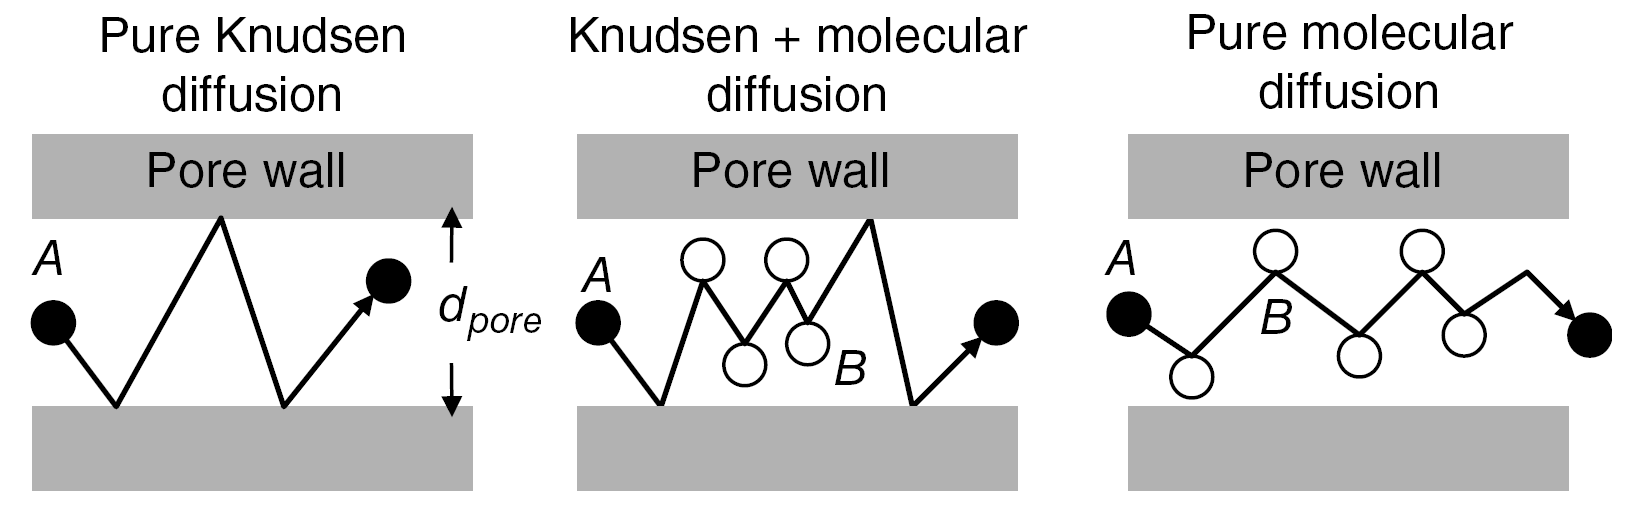
\includegraphics[width=12cm]{Knudsen-diffusion}
    \caption{Knudsen-diffusion}
\end{figure}

Knudsen扩散只适用于气体,因为液体分子的平均自由程非常小,通常接近分子本身的分子直径。Knudsen扩散系数的值与气相中扩散物质分子的平均自由程$ \lambda $有关,不同压力下的气体分子的平均自由程可用下式估算:

\begin{equation}
\lambda = \frac{1.0133\times10^{-3}}{p}
\end{equation}

其中,$ \lambda $为分子的平均自由程(\si{cm}),$ p $为压力(\si{\kPa})。

在孔径远大于分子的平均自由程时($ d_0>>\lambda $),扩散不受孔径的影响,主要发生Fick扩散,分子与孔壁的碰撞是可以忽略的。一旦孔径小到一定程度(通常是与分子的平均自由程相当或更小,如$ d_0/\lambda<0.1 $),分子与孔壁的碰撞成为主导,质量传递由Knudsen扩散决定。从气体动力学理论导出自扩散系数,

\begin{equation}
D_{AA} = \frac{\lambda u}{3} = \frac{\lambda}{3} \sqrt{\frac{8k_B NT}{\pi M_A}}
\end{equation}

由于发生Knudsen扩散时,分子现在更有可能与孔壁发生碰撞,而不是另一个分子,所以直接间分子平均自由程替换为孔径$ d_0 $,然后带入$ k_B $和$ N $这两个常数的值,得,

\begin{gather}
D_k = 4850d_0\sqrt{\frac{T}{M}}
\end{gather}

其中,$ D_k $为克努森扩散系数(\si{cm\squared\per\second}),$ T $为温度(\si{\kelvin}),$ M $为扩散物质的相对分子质量,无量纲。Knudsen扩散系数与孔径$ d_0 $和温度$ T $成正比,与气体摩尔质量$ M $成反比。这意味着小分子气体会表现出很高的扩散率。与Fick扩散不同,\textbf{Knudsen扩散与压力无关}。

\section{综合扩散}

一般来说,Knudsen扩散过程只有在低压和小孔径时才其主导作用,但在有些情况下,Knudsen扩散和分子扩散都很重要的。在给定的孔道中,如果分子扩散和克努森扩散同时存在,即$ 0.1<d_0/\lambda<100(0.01<Kn<10) $时,分子与分子间碰撞以及分子与孔壁间碰撞形成的扩散\textit{阻力}均不可忽略,称为综合扩散。使用下式计算综合扩散系数:

\begin{equation}
\frac{1}{D} = \frac{1}{D_k} + \frac{1}{D_{AB}}
\end{equation}

\section{多孔介质中的有效扩散系数}

基于Fick定律推导的扩散系数仅仅适合笔直的孔隙结构,而工业催化剂孔隙结构复杂,分子扩散路径更长,通常引入曲折因子来修正扩散路径的长度,即$ L_{porous}=\tau L $。

多孔介质催化剂任意界面的截面积为$ S\varepsilon $,扩散路径的长度为$ \tau L $,则单位时间内通过截面积的物质的量为:

\[ \frac{dn}{dt} = -DS\varepsilon\frac{dc}{d\tau L} = -D\frac{\varepsilon}{\tau}S\frac{dc}{d} \]

定义有效传质系数为:

\begin{equation}
D_e = \frac{\varepsilon}{\tau}D
\end{equation}

催化剂的孔隙率和曲折因子均可以通过实验来测定,一般情况下,$ \varepsilon=0.4\sim0.5 $,$ \tau=1\sim7 $。

\section{Thermal Diffusion/Soret effect}

由温差引起的扩散称为\textbf{Soret效应},也称热泳(\url{https://en.wikipedia.org/wiki/Thermophoresis})。当混合物温差大、分子质量相差大时会产生热扩散,分子质量高的物质在低温区域积累,分子质量低的物质在高温处积累。多组分混合物所有热扩散系数之和为0:

\begin{equation}
\sum_{i=1}^Q D_i^T = 0
\end{equation}

\section{球形扩散方程}

设球形催化剂的半径为$ R $,并处于连续流动的气流中,取半径为$ r $,厚度为$ dr $的一个体积微元进行质量恒算。即,质量随时间的变化=扩散进入体积微元的量-扩散出体积微元的量。

\[ \frac{\partial \left(4\pi r^2\Delta r c\right)}{\partial t} = \left( 4\pi r^2 N \right)_r - \left( 4\pi r^2 N \right)_{r+\Delta r} \]

对于稳态扩散,质量随时间的变化为0,即:

\[ \left( 4\pi r^2 N \right)_r - \left( 4\pi r^2 N \right)_{r+\Delta r} = 0 \]

展开,并除以球形壳的体积$ 4\pi r^2 \Delta r $,得:

\[ \frac{\left( 4\pi r^2 N \right)_r - \left( 4\pi r^2 N \right)_{r+\Delta r}}{4\pi r^2 \Delta r} = 0 \]

\[ \frac{(r^2 N)_r - \left(r^2 N\right)_{r+\Delta r}}{r^2\Delta r} = 0 \]

\[ \frac{r^2 N - (r^2+2r\Delta r + (\Delta r)^2)N}{r^2\Delta r} = 0 \]

约去相同得项后:

\[ \frac{-2r\Delta r N - (\Delta r)^2 N}{r^2\Delta r} = 0 \]

将$ \Delta r $换为$ dr $,并略去高阶无穷小项$ (\Delta r)^2 $

\[ \frac{1}{r^2}\frac{-d\left(r^2 N\right)}{dr} = 0 \]

将Fick定律得通量定义$ N=-D\frac{dc}{dr} $带入式中:

\[ \boxed{\frac{1}{r^2}\frac{-d\left(r^2 D\frac{dc}{dr}\right)}{dr} = 0} \]

按微积分基本法则也可展开为:

\begin{equation}\label{sphere_diffusion}
\boxed{D\left(\frac{d^2c}{dr^2} + \frac{2}{r} \frac{dc}{dr}\right) = 0}
\end{equation}

方程的边界条件为:

\[ r=R, c=c_0 \]
\[ r=0, c=0 \]

\section{浓物质传递}
由$i$个物质构成的,有$j$个反应的反应流、浓物质系统的质量守恒方程为:

\begin{equation}
    \frac{\partial}{\partial t}(\rho\omega_i) + \nabla\cdot(\rho\omega_i\bm{u}) = -\nabla\cdot\bm{j}_i + R_i
\end{equation}

其中$\omega_i$表示$i$物质的质量分数,$\bm{j}_i$为质量通量(mass flux)源项,表示分子扩散、电场迁移、热扩散等引起的通量。

\subsection{Maxwell-Stefan Description}
\textbf{Maxwell-Stefan}是最详细的扩散模型,计算消耗最大,是一个扩散占主导的模型。多组分混合物中,相对于质量平均速度的质量通量可使用通用的Fick方程定义,总的扩散通量依赖于物质的浓度梯度、温度、压力和外部驱动力:

\begin{equation}
    \bm{j}_i = -\rho\omega_i\sum_{k=1}^{Q} \tilde{D}_{ik} \bm{d}_{k} - D_i^T\nabla\ln T
\end{equation}

$\tilde{D}_{ik}$是多组分Fick扩散系数,$D_i^T$是热扩散系数,$\bm{d}_k$是扩散驱动力。对理想气体而言,扩散驱动力可表示为:

\begin{equation}
    \bm{d}_k = \frac{1}{cR_gT} \left[ \nabla p_k-\omega_k\nabla p - \rho_k \bm{g}_k +\omega_k \sum_{l=1}^{Q} \rho_l \bm{g}_l \right]
\end{equation}

其中,$p_k$为气体分压,$\rho_k$为物质$k$的密度,$\bm{g}_k$为作用于物质$k$的外部作用力(例如电场)。

\subsection{Mixture-Averaged Approximation}
\textbf{Mixture-Averaged}模型假定分压和温度变化对多组分扩散的影响可以忽略,假定由分子扩散引起的质量通量符合Fick定律,则分子扩散通量正比于摩尔分数的梯度,定义为:

\begin{gather}
    \bm{j}_{md,i} = -\rho_i D_i^m \frac{\nabla x_i}{x_i} \\
    \bm{j}_{md,i} = -\left( \rho D_i^m \nabla \omega_i + \rho \omega_i D_i^m \frac{\nabla M}{M} \right) \\
    \rho_i = \rho\omega_i, x_i = \frac{\omega_i}{M_i} M
\end{gather}

其中,混合物平均扩散系数定义为:

\begin{equation}
    D_i^m = \frac{1-\omega_i}{\sum_{k\neq i}^N \frac{x_k}{D_{ik}}}
\end{equation}

\subsection{Fick's law}
\textbf{Fick's law}是一个通用的模型,通常用来描述分子扩散不占主导地位的系统,不需要多组分扩散系数,计算消耗最低。

\section{化学吸附}
化学吸附只能发生在固体表面的活性位点$ \sigma $上,定义被A覆盖的活性位点与总活性位点之比为吸附率,剩下的为空位率:

\begin{gather}
    \theta_A = \frac{\sigma_A}{\sigma} \\
    \theta_V = 1-\theta_A
\end{gather}

分子的吸附速率$ r_{ads} $与表面空位率和气体分压成正比,解吸率与表面占有率成正比:

\begin{gather}
    r_{ads} = k_{ads}p_A\theta_V \\
    r_{des} = k_{des}\theta_A
\end{gather}

达到吸附平衡时,表观速率$ r=r_{ads}-r_{des}=0 $,有:

\[k_{ads}p_A(1-\theta_A)=k_{des}\theta_A\]

令$ K_A=\frac{k_{ads}}{k_{des}} $,称为\textbf{吸附平衡常数},得\autoref{Langmuir},称为Langmuir吸附等温式:

\begin{equation}\label{Langmuir}
    \theta_A = \frac{K_Ap_A}{1+K_Ap_A}
\end{equation}

为了根据本体浓度$ c $和表面浓度$ cs $来建立传递和反应方程,执行以下代换,其中$ \Gamma_s $为表面得最大吸附浓度:

\[\theta_A = c_s/\Gamma_s\]
\[p_A=cRT\]

将得到下式,粗体为吸附和脱附反应速率常数。

\begin{gather}
    r_{ads} = \bm{\frac{k_{ads}RT}{\Gamma_s}}c(\Gamma_s-c_s)\\
    r_{des} = \bm{\frac{k_{des}}{\Gamma_s}}c_s
\end{gather}

对于表面来讲,涉及表面扩散、吸附脱附、表面反应,质量守恒为:

\begin{equation}
    \frac{\partial c_s}{\partial t}+\nabla\cdot(-D_s\nabla c_s) = r_{ads}-r_{des}=R
\end{equation}

本体溶液的质量守恒用经典的对流扩散方程描述:

\begin{equation}
    \frac{\partial c}{\partial t} + \nabla\cdot(-D\nabla c+\bm{u}c) = R
\end{equation}

\section{表面反应Surface reaction}

通常,表面反应中涉及两个浓度:一是吸附到反应性表面的物质的浓度,$ c_{s,i} $;二是反应性表面上与表面反应相关的固体物质的浓度,$ c_{b,k} $。对本体物质来讲,用\textbf{法向通量}表示物质被吸附到反应性表面上;对表面物质来讲,使用\textbf{切向通量}$ N_{t,i} $表示表面物质在表面上的迁移(迁移的方式通常只有扩散,其中$ D_{s,i} $表示表面扩散系数,\si{\meter\squared\per\second})。

\begin{equation}
N_{t,i} = -D_{s,i}\nabla_t c_{s,i}
\end{equation}

整个反应性表面上的质量传递控制方程写做:

\begin{equation}\label{key}
\frac{\partial c_{s,i}}{\partial t} = -\nabla\cdot N_{t,i} + R_{s,i}
\end{equation}

其中,$ R_{s,i} $是由表面反应、吸附/解吸引起的物质源项,\si{\mole\per\meter\squared\per\second}。

在表面反应动力学中,通常最感兴趣的是表面覆盖分数(the fractional surface coverages),$ \theta_i $,无量纲,定义为:

\begin{equation}
\theta_i = \frac{\sigma_i c_{s,i}}{\Gamma_s}
\end{equation}

其中,$ \Gamma_s $为表面位点密度,即单位面积上对物质的最大的吸附量,\si{\mole\per\meter\squared};$ \sigma_i $为各物质的位点占有数,无量纲。

\section{多孔介质质量传递}

对每一个组分应用质量守恒定律,并忽略源汇项,得出基于质量浓度的\textbf{单组分质量守恒方程}:

\begin{equation}
\frac{\partial \rho_i}{\partial t} + \nabla\cdot(\rho_i\bm{U_i}) = 0
\end{equation}

将方程中的质量浓度和内在平均速度汇总,得出全部组分的质量守恒方程:

\begin{equation}
\frac{\partial \rho}{\partial t} + \nabla\cdot(\sum\rho_i\bm{U_i}) = 0
\end{equation}

使用$ \bm{U}=\frac{1}{\rho}\sum\rho_i\bm{U_i} $表示质量平均速度,得出:

\begin{equation}
\frac{\partial \rho}{\partial t} + \nabla\cdot(\rho\bm{U}) = 0
\end{equation}

我们定义物质$ i $相对于质量平均速度的运动为扩散(diffusion),$ \bm{U_i}-\bm{U} $为扩散速度,则扩散通量为:

\begin{equation}
\bm{j_i} = \rho_i(\bm{U_i} - \bm{U})
\end{equation}

则,考虑对流-扩散的单组分质量守恒方程为:

\begin{equation}
\frac{\partial \rho_i}{\partial t} + \nabla\cdot(\rho_i\bm{U}) = -\nabla\cdot \bm{j_i}
\end{equation}

根据Fick定律,$ \bm{j_i} = -D\nabla\rho $,在上式两端同时乘上孔隙率$ \varepsilon $以考虑多孔介质内的质量传递:

\begin{equation}
\varepsilon\frac{\partial \rho_i}{\partial t} + \varepsilon\nabla\cdot(\rho_i\bm{U}) = \varepsilon\nabla\cdot(D\nabla \rho_i)
\end{equation}

运用Dupuit–Forchheimer relationship,考虑多孔介质内部的有效扩散系数,并将上式改写为关于摩尔浓度:

\begin{equation}
\varepsilon\frac{\partial c_i}{\partial t} + \varepsilon\nabla\cdot(c_i\bm{u}) = \varepsilon\nabla\cdot(D_{eff}\nabla c_i)
\end{equation}

\section{化学反应}

化学反应速率表达式一般为:

\begin{equation}
\frac{dc}{dt} = -kc^n
\end{equation}

反应速率常数常常于温度和和活化能相关,一般由Arrhenius relationship给出:

\begin{equation}
k = A \exp(-\frac{E}{RT})
\end{equation}

和温度相关的Arrhenius表达式一般为:

\begin{equation}
k = A \left( \frac{T}{T_{ref}} \right) \exp(-\frac{E}{RT})
\end{equation}

\section{蒸汽压}

通常,蒸气压随着温度的升高而增加。然而,蒸汽压力的温度依赖性并不是线性的。液体的饱和蒸汽压由Clausius–Clapeyron equation控制:

\begin{equation}
\frac{dp}{dT} = \frac{\Delta H_{vap}}{T\Delta V_m}
\end{equation}

其中,$ \Delta H_{vap} $为蒸发焓,$ \Delta V_m $为相变摩尔体积变化。众所周知,蒸汽的体积$ V_g $远大于等效液体的体积。因此,使用蒸汽体积表示相变摩尔体积变化也是合理的,同时结合理想气体状态方程,可将Clausius–Clapeyron equation改写为:

\begin{equation}
\frac{d\ln p}{dT} = \frac{\Delta H_{vap}}{RT^2}
\end{equation}

\section{不连续的界面边界条件}

通常情况下,界面处边界条件为固定值或者指定通量。但是,传质比传热更复杂的现象是,在两种材料之间的界面处物质浓度是不连续的,而温度是连续的。举一个熟悉的例子,考虑一个暴露在空气中的水池。如果我们对确定水蒸气传递到空气中的速率感兴趣,界面处的气相浓度应该由Raoult’s law指定,

\[ p_i = x_i p \]

同理,吸收和解析系统应该由Henry’s law确定,

\[ x_i = \frac{p_i}{H} \]










